\subsection{Auswertung der Schwellenkurve}
In Tab. \ref{tab:schwelle} sind die Anzahl der Ereignisse in den Detektoren in Abhängigkeit der Schwellenspannung $U_S$ aufgeführt. 

\begin{table}
\centering
\caption{Anzahl der Ereignisse in Abhängigkeit der Schwellenspannung $U_S$}
\label{tab:schwelle}
\begin{tabular}{cccccc}
\toprule
$U_S$/\si{\milli\volt}& D12 & D23, D24, D1 oder D2 & D25 & Koinzidenzen & Koinzidenzen/D25\\
\midrule
-50 & 4384 & 14259 & 14639 & 122 & 0.0083\\
-60 & 3631 & 14225 & 14526 & 128 & 0.0088\\
-70 & 3181 & 14401 & 14642 & 121 & 0.0083\\
-80 & 2773 & 14517 & 14848 & 92 & 0.0062\\
-90 & 2322 & 14701 & 15644 & 108 & 0.0069\\
-100 & 2024 & 14425 & 15026 & 82 & 0.0055\\
-110 & 1649 & 14488 & 15122 & 67 & 0.0044\\
-120 & 1551 & 14479 & 15370 & 65 & 0.0042\\
-130 & 1339 & 14618 & 15239 & 61 & 0.0040\\
-140 & 1286 & 14424 & 15481 & 66 & 0.0042\\
-150 & 1129 & 14291 & 14912 & 45 & 0.0030\\
-160 & 1028 & 14641 & 14964 & 50 & 0.0033\\
-170 & 922 & 14583 & 14668 & 45 & 0.0031\\
-180 & 823 & 14595 & 14834 & 36 & 0.0024\\
-190 & 725 & 14567 & 15234 & 36 & 0.0024\\
-200 & 679 & 14571 & 14761 & 26 & 0.0018\\
-210 & 605 & 14527 & 14916 & 37 & 0.0025\\
-220 & 545 & 14649 & 15183 & 21 & 0.0014\\
-230 & 483 & 14591 & 14850 & 20 & 0.0013\\
-240 & 450 & 14652 & 14996 & 24 & 0.0016\\
-250 & 366 & 14678 & 14807 & 15 & 0.0010\\
\bottomrule
\end{tabular}
\end{table}

Die Koinzidenzen wurden auf die Anzahl der Ereignisse in D25 normiert, um Schwankungen in der Höhenstrahlung auszugleichen. In Abb. \ref{fig:schwelle} ist dies über der Schwellenspannung aufgetragen. Die optimale Schwellenspannung liegt nun bei dem Wendepunkt der Kurve. Leider kann man keinen Wendepunkt erkennen, da die Daten stark streuen. Bei etwa $U_S = (-140 \pm 10)\si{\milli \volt}$ kann aber einen leichten Knick ausmachen. Deswegen haben wir beschlossen, die Schwellenspannung auf 140\si{\milli \volt} zu setzen.

\begin{figure}
\centering
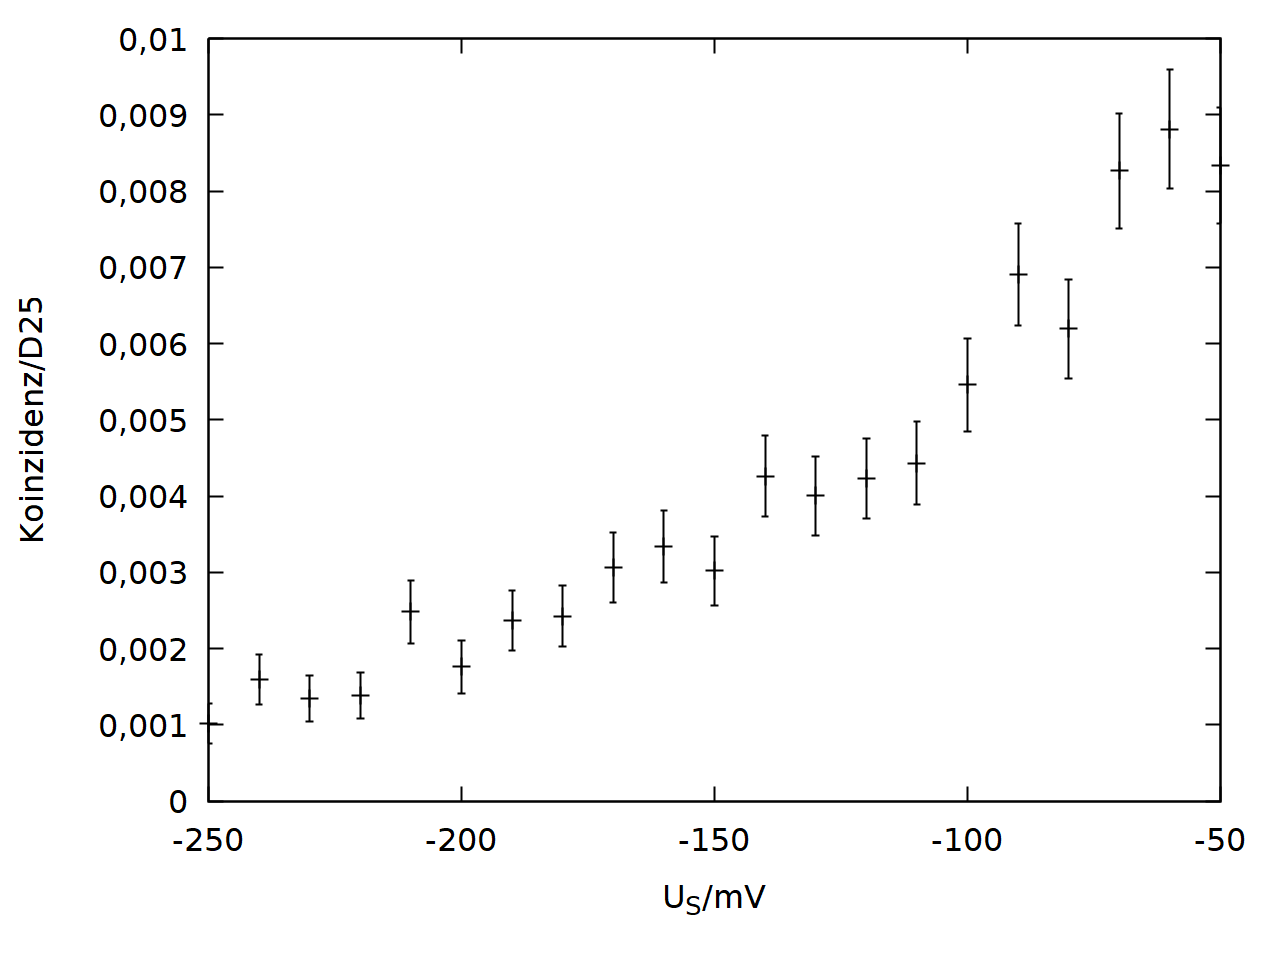
\includegraphics[width=0.75\linewidth]{data/friedrich/schwelle.png}
\caption{Koinzidenzen/D25 über der Schwellenspannung $U_S$}
\label{fig:schwelle}
\end{figure}

\subsection{Auswertung der Winkelmessung}
In Tab. \ref{tab:winkel} ist das Ergebnis der Winkelmessung eingetragen. Die Messung dauerte 1126731 \si{\second}. Dabei gab es 0 zeitliche Zufallskoinzidenzen und 1239 räumliche Zufallskoinzidenzen. Die zeitlichen Zufallskoinzidenzen sind also vernachlässigbar. Da man keine weiteren Informationen darüber hat, ob die räumlichen Zufalls-Koinzidenzen die Zahl gemessenen Teilchen erhöht oder verringert, wird für alle Messwerte ein Fehlerintervall von $\pm 1239$ Koinzidenzen angenommen. Da man die anderen Fehler auf die Anzahl der Koinzidenzen (in den Detektoren und der Elektronik) nicht abschätzen kann, ist dies auch der einzige Fehler, der in die Auswertung einfließt\footnote{Der rein statistische Fehler ist bei $N$ Ereignisse etwa $\sqrt{N} \leq 100$, also deutlich kleiner als 1239}. Als Fehler für den Winkel wird $\Delta \phi = 7,5^\circ$ angenommen, da die Detektoren jeweils einen Winkelbereich von $15^\circ$ abdecken.\\ 

\begin{table}
\centering
\caption{Messwerte Winkelmessung}
\label{tab:winkel}
\begin{tabular}{ccc}
\toprule
Winkel $\phi/^\circ$& Detektorkombination & Ereignisse\\
\midrule
0 &	24-25-12	&6694\\
15&	1-25-13	&8357\\
30&	2-25-14	&7928\\
45&	3-25-15	&4444\\
60&	4-25-16	&1588\\
75&	5-25-17	&345\\
90&	6-25-18	&6\\
-75&7-25-19	&582\\
-60&8-25-20	&2379\\
-45&9-25-21	&37\\
-30&10-25-22	&7302\\
-15&11-25-23	&5491\\
\bottomrule
\end{tabular}
\end{table}

In Abb. \ref{fig:winkel} ist die Anzahl der Koinzidenzen über $\phi$ dargestellt.

\begin{figure}
\centering
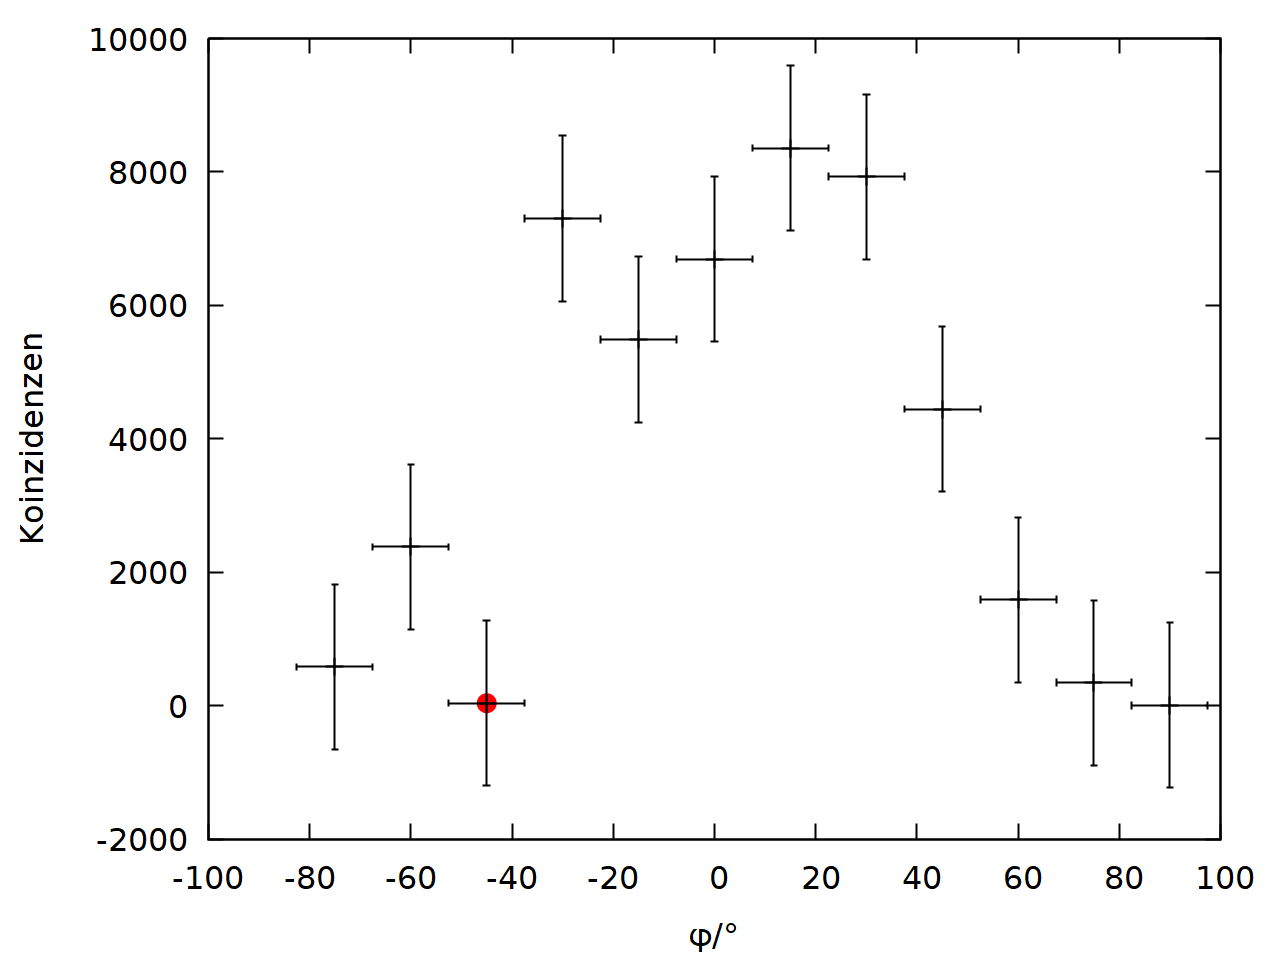
\includegraphics[width=0.75\linewidth]{data/friedrich/winkel.png}
\caption{Koinzidenzen in Abhängigkeit vom Winkel $\phi$}
\label{fig:winkel}
\end{figure}

Die Verteilung ist (etwa innerhalb der Fehlergrenzen) symmetrisch. Nur der Wert für $-45^\circ$ beträgt 37 (roter Kreis), während der Wert für $45^\circ$ 4444 beträgt. Da diese Abweichung ein vielfaches des angenommenen Fehlers ist und der Wert 37 auch im Vergleich zu den benachbarten Werten deutlich kleiner ist, wird angenommen, dass dieser Wert durch eine fehlerhafte Messapparatur zustande kommt. Er wird also als grober Fehler gewertet und wird für die weitere Auswertung nicht beachtet.\\

Es wird jetzt getestet, ob die Winkelverteilung durch eine $\cos^2{\phi}$ beschrieben werden kann. Dazu werden die Koinzidenzen über $\cos^2{\phi}$ aufgetragen und ein linearer Fit $a\cdot x + b$ (mittels Gnuplot) durchgeführt. \\

\begin{figure}
\centering
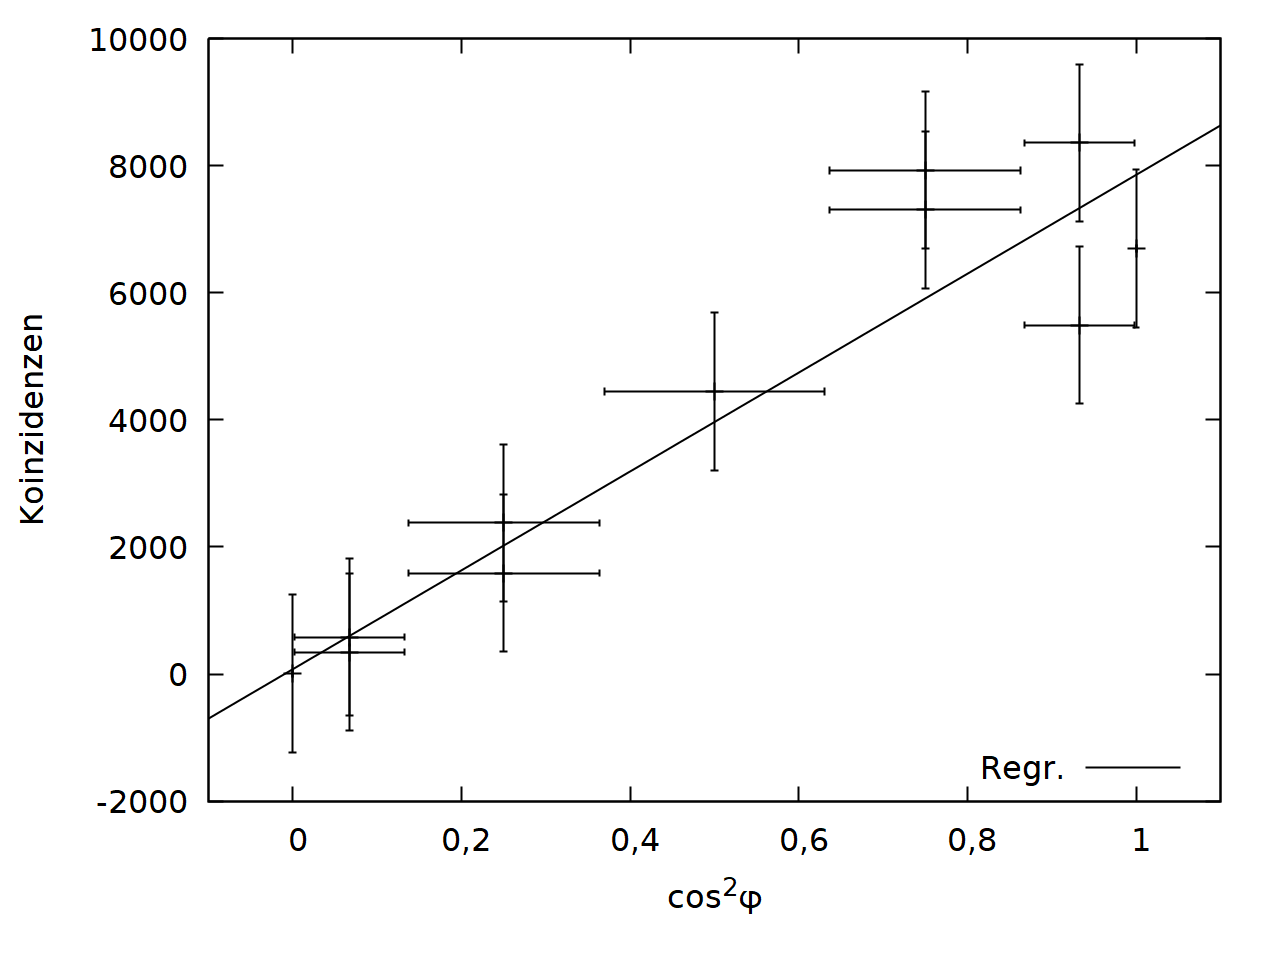
\includegraphics[width=0.75\linewidth]{data/friedrich/winkel_cos.png}
\caption{Koinzidenzen in Abhängigkeit von $\cos^2{\phi}$ mit linearem Fit}
\label{fig:winkel_cos}
\end{figure}

\begin{figure}
\centering
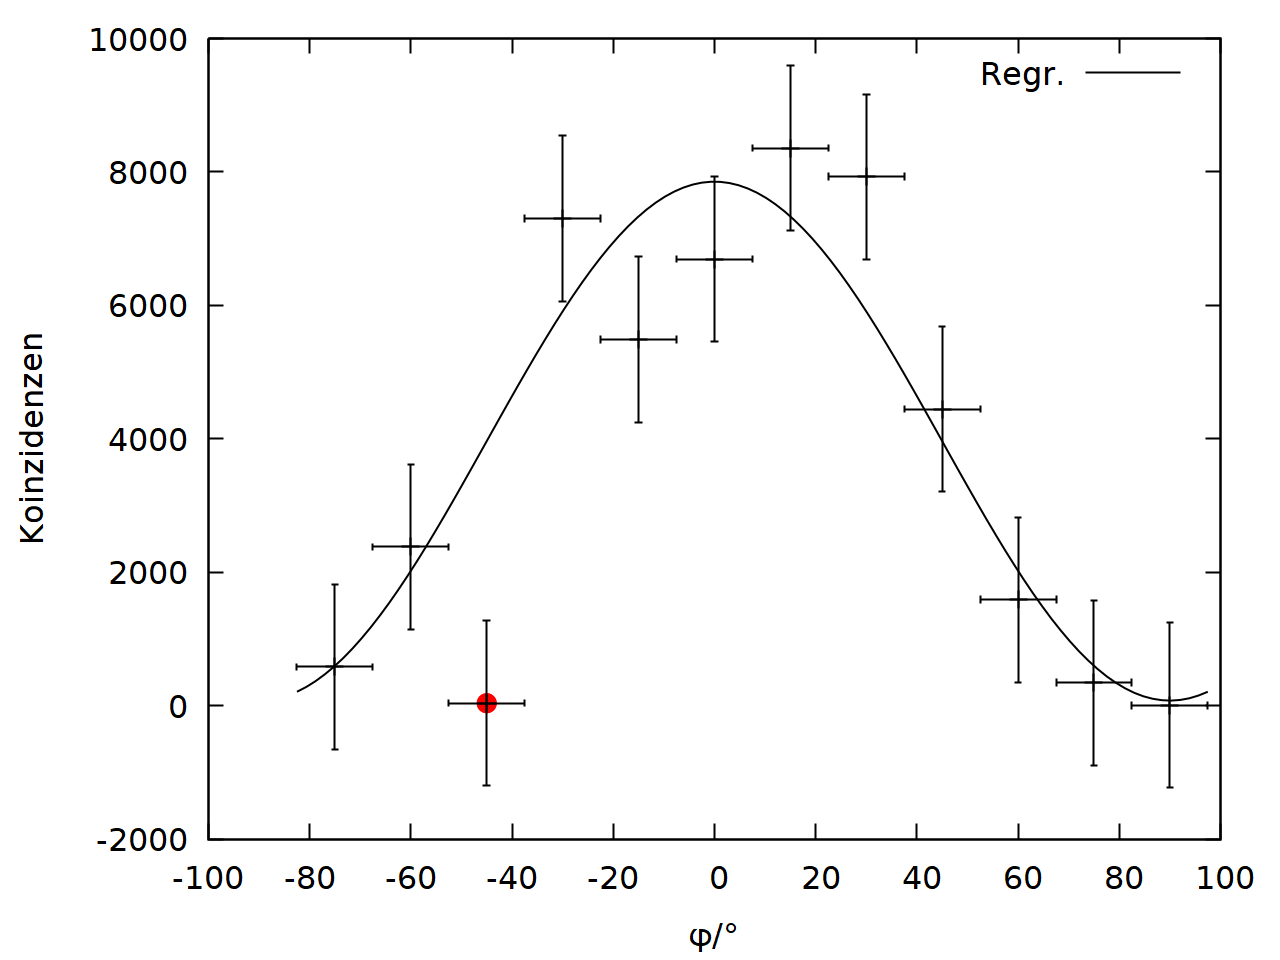
\includegraphics[width=0.75\linewidth]{data/friedrich/winkel_ges.png}
\caption{Koinzidenzen in Abhängigkeit vom Winkel $\phi$ mit $\cos^2{\phi}$-Fit}
\label{fig:winkel_ges}
\end{figure}

Der Fit ergibt: $a = (7,7 \pm 0,9)\cdot 10^3$ und $b = 80 \pm 570$. In Abb. \ref{fig:winkel_cos} ist zu erkennen, dass die Daten auch etwa auf dieser Fitgerade liegen. Ein linearer Fit ist also berechtigt. Der Achsenabschnitt $b$ kann im Rahmen des Fehlers 0 sein. In diesem Experiment kann man also nicht feststellen, ob es einen Offset auf der $\cos^2{\phi}$-Verteilung gibt.\\

In Abb. \ref{fig:winkel_ges} wurde die ($a \cdot \cos^2{\phi} + b$)-Funktion in die Daten eingetragen. Hier kann man erkennen, dass der  $\cos^2{\phi}$-Fit eine gute Näherung für große $\phi$ ist. Für kleine $\phi$ weichen die Daten z.T. aus den Fehlergrenzen ab, bzw. liegen nur knapp in den Fehlergrenzen. Diese Abweichungen lassen sich nicht einfach durch Statistik erklären, da diese Fehler im Bereich von $\sqrt{N} \leq 100$ sind. Somit müssen entweder weitere Fehlerquellen im Messsystem sein oder eine $\cos^2{\phi}$-Verteilung eignet sich nicht zur Beschreibung der Winkelverteilung für kleine $\phi$.\\

Geht man davon aus, dass die Verteilung symmetrisch für $\phi$ und $-\phi$ sein soll, so kann man als Maß für den Fehler die Differenz zwischen Koinzidenzen bei gegenüberliegenden Winkeln nehmen. Die größte Abweichung gibt es bei $\phi = -15^\circ,15^\circ$. Sie beträgt: $8357
 - 5491 = 2866$, also mehr als doppelt so viel wie die Zufallskoinzidenzen. Mit diesem Fehler würden alle Punkte im Fehlerbereich liegen. Somit ist eine $\cos^2{\phi}$-Verteilung auch in diesem Bereich realistisch. Man kann also die Winkelverteilung durch eine $\cos^2{\phi}$-Verteilung annähern, allerdings gibt es für kleine $\phi$ starke Schwankungen.\\
 
\subsection{Zufallskoinzidenzen}
Im Detektor Z25 gab es $N = 74678$ Koinzidenzen\footnote{Wir wissen nicht wie viele Koinzidenzen in nur zwei Detektoren gab. Die Zahl der Ereignisse in Z25 ist aber definitiv eine obere Schranke dazu. Eine untere Schranke sind z.B. die Dreierkoinzidenzen in Z14-Z25-Z2: $7928$}. Die Messdauer war $t = 1126731 \si{\second}$. Damit ergibt sich nach \ref{equ:random_space} und \ref{equ:random_time}:\\
\begin{align*}
N_{\text{raum}} &= 7 \cdot 10^{-9}\\
N_{\text{zeit}} &= 5 \cdot 10^{-17}
\end{align*}  
 
\subsection{Auswertung der Energieverteilung}

Die Daten für diese Auswertung erhielten wir von den Tutoren, da sowohl wir als auch die Tutoren das Starten des Programmes vergessen hatten.\\

\begin{figure}
\centering
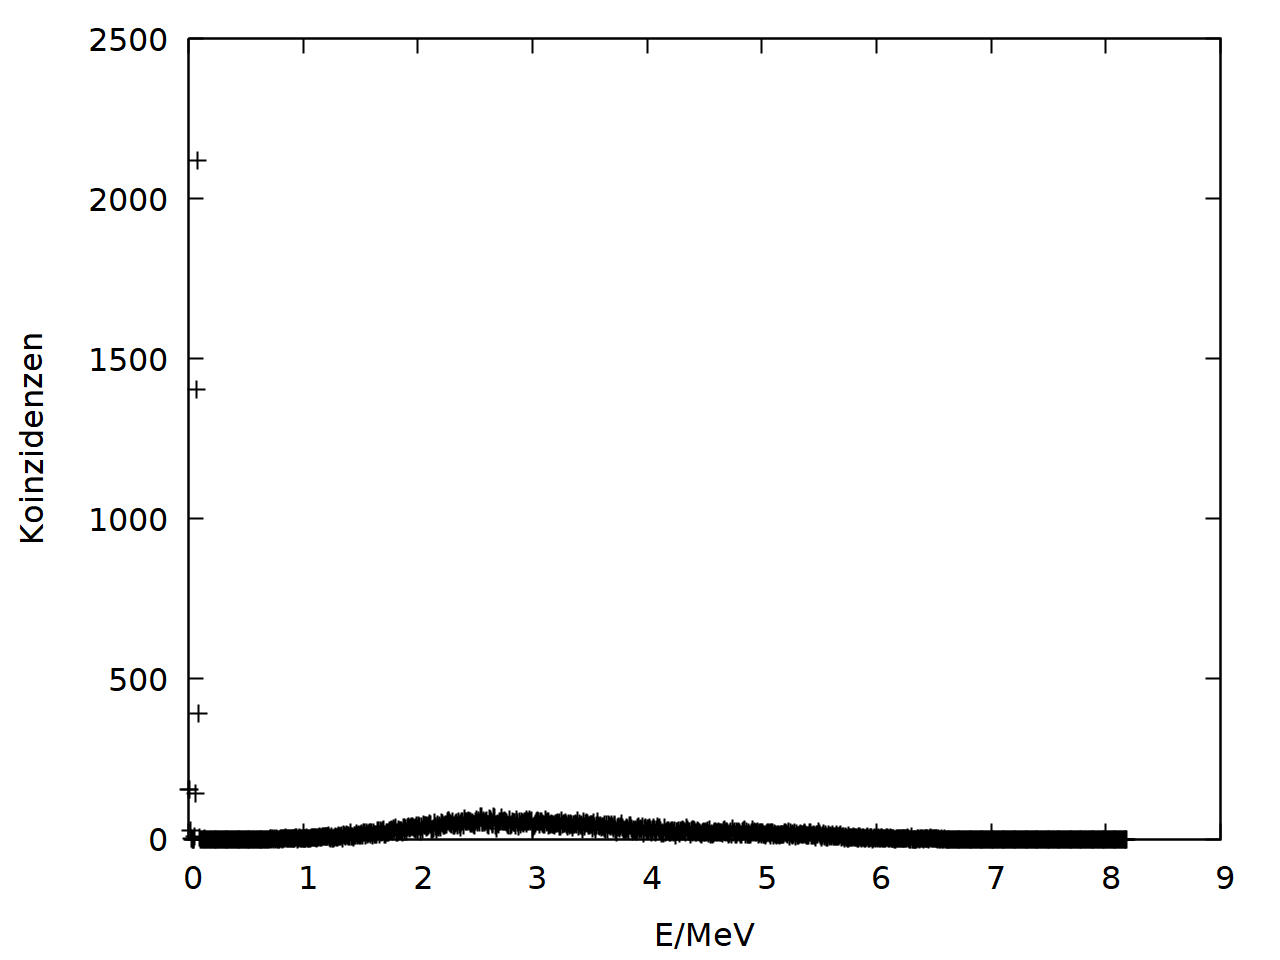
\includegraphics[width=0.75\linewidth]{data/friedrich/mca_raw.png}
\caption{Messwerte der Energieverteilung}
\label{fig:mca_raw}
\end{figure}

\begin{figure}
\centering
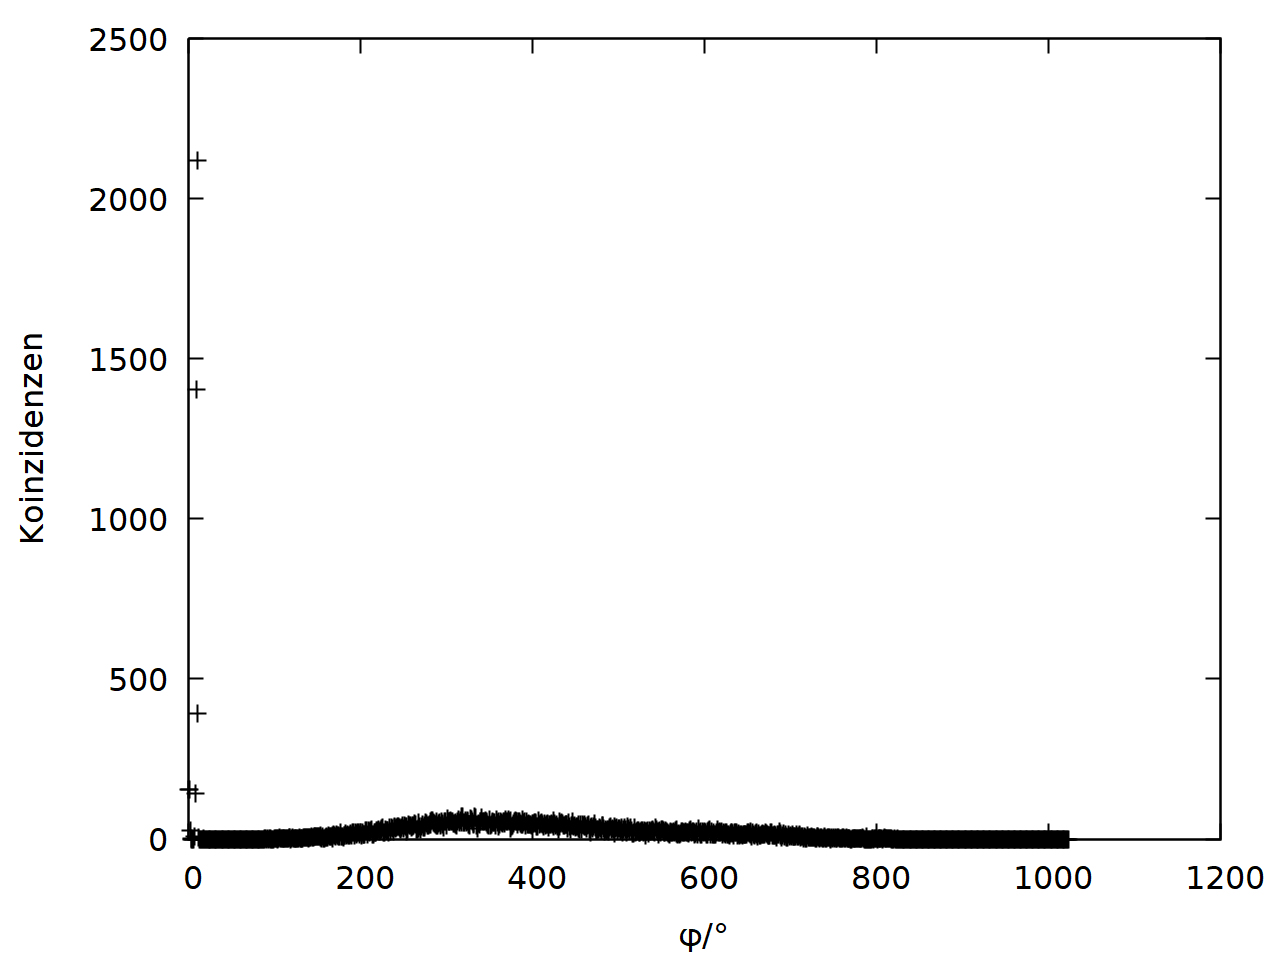
\includegraphics[width=0.75\linewidth]{data/friedrich/mca.png}
\caption{Fits an die Energieverteilung}
\label{fig:mca}
\end{figure}

In der Datei steht nur die Anzahl der Energieereignisse je Bin steht, aber nicht, wie groß ein Bin ist. Aus der Konfigurationsdatei wurde geschlossen, dass ein Bin 8keV groß ist ('calfact=8' und 'calunit=keV'). Das ist für die Auswertung auch nicht relevant, da es nur um die qualitative Energieverteilung geht.  

In Abb. \ref{fig:mca_raw} sind die gemessenen Werte abgebildet. Bei ganz kleinen Energien werden viele Ereignisse festgestellt (etwa in den ersten 20 Bins). Es wird sich dabei vermutlich um Untergrund handeln, der die Schwelle des Diskriminators überschnitten hat. Deswegen nehmen wir die ersten 20 Bins aus der Auswertung heraus. An die Daten wird jetzt sowohl eine Landauverteilung
\[A\exp{\left(-\frac{1}{2}((x-b)/l + e^{-(x-b)/l)}\right)}\] als auch eine Gaussverteilung gefittet

\[B\exp{\left(-\frac{1}{2}((x-c)/d)^2 \right)}\]
 (siehe Abb. \ref{fig:mca}). Das Ergebnis der Fits ist
 \begin{align}
 A &= 89 \pm 0,7\\
 b &= (2,664 \pm 0,008)\si{\mega\eV}\\
 l &= (0,665  \pm 0,006)\si{\mega\eV}\\
 B &= 51,4 \pm 0,5\\
 c &= (3,04\pm 0,01)\si{\mega\eV}\\
 d &=( 1,10 \pm 0,01) \si{\mega\eV}
 \end{align}
 
In Abb. \ref{fig:mca} kann man erkennen, dass die Landauverteilung deutlich besser die Messwerte annähert, als die Gaussverteilung. Nur bei großen Energien weicht die Landauverteilung von der Messung ab. Der lange Ausläufer der Landauverteilung existiert nicht, die Daten zeigen hier eher ein gaussförmiges Verhalten. Das liegt daran, dass die Landauverteilung nur eine gute Näherung für dünne Schichten ist, während die Gaussverteilung dicke Schichten beschreibt. Die verwendeten Detektoren haben eine Ausdehnung und können daher nicht vollständig durch eine Landauverteilung beschrieben werden. Deswegen hat die Verteilung keinen langen Schwanz.\\

Das Maximum der Landauverteilung liegt bei $b \approx 2,7\si{\mega\eV}$. Das ist in grober Übereinstimmung mit Abb. \ref{fig:landau}, wo das Maximum bei etwa $2,4\si{\mega\eV}$ ist. Die gemessene Energie ist also etwas größer als die theoretisch berechnete. Dabei ist aber zu beachten, dass es bei der theoretischen Berechnung viele unbekannte Größen gab, die nur abgeschätzt wurden. Die Differenz zwischen Theorie und Experiment ist also nicht unerwartet.